\documentclass[runningheads]{llncs}
\usepackage[T1]{fontenc}
\usepackage{booktabs,array,graphicx,placeins,hyperref,url}
\hypersetup{hidelinks}
\emergencystretch=2em
\newcommand{\code}[1]{\texttt{#1}}
% Generated from validated signoff bundles.
\newcommand{\DesignCount}{7}
\newcommand{\StageCount}{21}
\newcommand{\TestPasses}{955}
\newcommand{\TestSkipped}{15}
\newcommand{\CellMin}{16}
\newcommand{\CellMax}{1024}
\newcommand{\SetupMin}{4.911}
\newcommand{\HoldMin}{0.049}
\newcommand{\RuleCount}{211}
\newcommand{\ModelCalls}{1}
\newcommand{\ModelInputTokens}{6999}
\newcommand{\ModelOutputTokens}{1403}
\newcommand{\SourceShort}{af31b39f6782}
\newcommand{\InitialAluDRC}{1}
\newcommand{\PaddingBefore}{0}
\newcommand{\PaddingAfter}{2}
\newcommand{\ClockPeriod}{10.0}
\newcommand{\ClockUncertainty}{0.25}
\newcommand{\OutputLoad}{0.05}
\newcommand{\RepairRuntime}{168.8}
\newcommand{\RepairModel}{claude-sonnet-5}

% Generated from native attack, repair and repeat evidence.
\newcommand{\NativeAttackTrials}{18}
\newcommand{\NativeBlocked}{18}
\newcommand{\NativeFalseClean}{18}
\newcommand{\DegradedRuleCount}{152}
\newcommand{\StudyEpisodes}{9}
\newcommand{\StudyVerified}{7}
\newcommand{\StudyEscalated}{2}
\newcommand{\StudySuccessPct}{77.8}
\newcommand{\StudyEscalationPct}{22.2}
\newcommand{\StudyModelCalls}{20}
\newcommand{\StudyInputTokens}{174306}
\newcommand{\StudyOutputTokens}{50164}
\newcommand{\ProposalPromotions}{20}
\newcommand{\ConfirmedBadProposals}{11}
\newcommand{\UncheckedProposals}{2}
\newcommand{\TimingBefore}{-0.326192}
\newcommand{\TimingAfter}{0.001586}
\newcommand{\CounterStressWNS}{-0.715689}
\newcommand{\LargeCells}{1024}
\newcommand{\RepairSourceShort}{18d948815ac6}
\newcommand{\ExactRoutePairs}{6}
\newcommand{\NormalizedGDSPairs}{6}

% Generated from validated frozen cohorts.
\newcommand{\FrozenSourceShort}{af31b39f6782}
\newcommand{\ProposalSourceShort}{18d948815ac6}
\newcommand{\FrozenPrimaryPairs}{7}
\newcommand{\FrozenRawGDSPairs}{1}
\newcommand{\ArchivedTimingWrong}{11}
\newcommand{\ArchivedTimingWrongPct}{78.6}
\newcommand{\ArchivedTimingMissing}{2}
\newcommand{\TimingProposalCount}{14}
\newcommand{\FrozenTimingWrong}{14}
\newcommand{\FrozenTimingWrongPct}{100.0}

\title{Supplement: Candidate-Bound Evidence for RTL-to-GDS Signoff}
\titlerunning{RTL2GDSAGI: supplementary evidence}
\author{Rithwik Vallabhan TV \and Sreejeesh SG \and Jayaraj U Kidav \and Nanditha N Varma}
\authorrunning{R. Vallabhan TV et al.}
\institute{NIELIT Calicut, India}
\begin{document}\maketitle

\section{Source and Execution Ledger}
The primary manuscript uses frozen implementation \code{\FrozenSourceShort}
for fourteen design runs, twenty separate recorded-proposal executions,
eighteen fault-consistency executions, and a replayed spacing-repair episode.
The latter submits the recorded padding delta through a scripted proposal
adapter and makes zero new model calls. It encounters native spacing failure,
authorizes the recorded change, reruns the affected stages, and certifies.
It supplies the post-repair artifact used by the new swap fixture.

The twenty recorded proposals originate from live Claude Sonnet 5 runs
(Anthropic; identifier \code{claude-sonnet-5}) on snapshot
\code{\ProposalSourceShort}. The primary
replay counts those proposal states, with six frozen certifications and
fourteen native failures. It is separate from the original nine live episodes,
which produced seven certifications and two escalations on that earlier code.
Source snapshots, complete typed configurations, and commands identify both
phases. Current source is \code{\FrozenSourceShort}; Git commits modifying the
manuscript and drivers do not introduce a third implementation snapshot.

The 2x2x2 padding ablation retains four source interventions derived from the
frozen source. Their changes remove only the CTS and/or routing padding calls.
Worker count is the other declared factor. The mapped netlist and placed DEF
match across the CTS intervention, while CTS and downstream artifacts differ.
The main frozen renderer retains both padding calls.

\section{Original Live Repair Episodes}
Three episodes per fixture type were declared before execution. Spacing and
PDN each certify in 3/3 episodes; timing certifies in 1/3. The original twenty
model responses record 174306 input tokens and 50164 output tokens. Table~\ref{tab:episodes}
retains every episode. These observations belong to \code{\ProposalSourceShort}.
They are descriptive outcomes for repeated fixtures, with no population
repair-rate estimate.
\begin{table}[htbp]\centering\small\setlength{\tabcolsep}{4pt}
\caption{All nine original live repair episodes on source 18d948815ac6. These archived outcomes are separate from frozen replay and larger episodes.}\label{tab:episodes}
\begin{tabular}{@{}lllll@{}}\toprule
Episode & Initial failure & Final evidence & Calls & Outcome \\
\midrule
Spacing 1 & 1 marker & Full signoff & 1 & Verified \\
Spacing 2 & 1 marker & Full signoff & 1 & Verified \\
Spacing 3 & 1 marker & Full signoff & 1 & Verified \\
PDN 1 & PDN-0185 & Full signoff & 1 & Verified \\
PDN 2 & PDN-0185 & Full signoff & 1 & Verified \\
PDN 3 & PDN-0185 & Full signoff & 1 & Verified \\
Setup 1 & -0.326192 ns & 0.001586 ns & 2 & Verified \\
Setup 2 & -0.326192 ns & Not certified & 3 & Escalated \\
Setup 3 & -0.326192 ns & Not certified & 9 & Escalated \\
\bottomrule\end{tabular}\end{table}


The original timing sequence at unchanged 3 ns is shown in
Figure~\ref{fig:archivedtiming}. The successful configuration repeats three
times at +1.586 ps under its archived source and three times at $-0.654$ ps
under the frozen implementation. The current-source failure is retained;
the primary factorial experiment measures the effect of CTS padding rather
than attributing the result to uncontrolled noise.
\begin{figure}[htbp]\centering
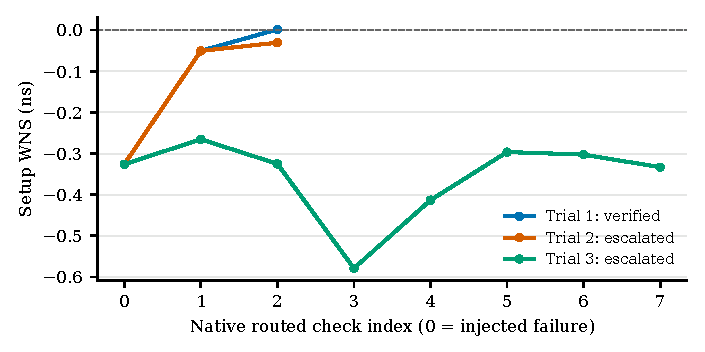
\includegraphics[width=.88\linewidth]{figures/timing_stress.pdf}
\caption{Archived native routed timing checks at 3 ns on source 18d948815ac6. Lines end at the last completed check, including escalated episodes.}
\label{fig:archivedtiming}\end{figure}

The archived class replay gives spacing 0/3 failed states, PDN 0/3, and timing
11/14, with two additional timing states lacking a completed target check.
Every confirmed failure in the earlier 11/20 headline is therefore from the
timing fixture. Fresh native execution establishes outcomes for all twenty
states on the frozen source: spacing 0/3 failures, PDN 0/3, and timing 14/14.
No unavailable target is silently counted as a confirmed archived failure.

\section{Complete-State Replay Reconstruction}
Reconstruction starts with the archived IR defaults and applies the logged
characterization seed, initial overrides, curated numerical changes, and all
accepted model deltas in temporal order. The archived renderer used the
native one-worker default; the current replay declares that effective count
explicitly. The reconstructed final IR matches every archived successful
episode before any new native execution. Fresh runs disable further repair.

An initial reconstruction pilot omitted the curated PDN changes preceding
the model call: strap offset 50 to 21.42~$\mu$m and utilization 0.35 to 0.29.
Its three PDN configurations did not represent the recorded promoted states.
The complete pilot and original launcher remain in the archive and are excluded
from the final twenty-state result. The corrected cohort was declared and
executed separately, with the full-state equality checks described above.
This exclusion corrects configuration reconstruction rather than selecting
favorable native outcomes.

\section{Native Checker Invocation Controls}
The pinned OpenLane wrapper and public source bytes match. The installed
modern PDK deck expects runtime rule flags that this wrapper does not forward.
The previous pairing declares zero categories and zero markers for both known
violating and clean synthetic geometry. It is an inactive configuration
observation and is excluded as an active-DRC baseline.

Table~\ref{tab:drccontrols} reports active paired controls. The legacy native
deck reports 166 categories and metal/off-grid violations; its tested poly
category is absent. The modern PDK options and explicit adapter each report
220 categories, with metal/poly/off-grid markers 3/1/4 and paired clean counts
0/0/0. These control counts are raw inventories for those configurations, not
the primary controller's 211 normalized-category contract. Violating stage
calls return zero despite markers, so marker reporting and native exit rejection
are distinguished. The adapter is a recorded sidecar change, not an unmodified
stock full-flow run.
\begin{table}[htbp]\centering\small\setlength{\tabcolsep}{4pt}
\caption{Paired synthetic DRC controls. Marker columns list metal/poly/off-grid fixtures. Modern controls use the PDK runtime options; the adapter is an explicit sidecar change. The inactive prior wrapper is a configuration diagnostic, excluded from this active-checker table.}\label{tab:drccontrols}
\begin{tabular}{@{}lrrr@{}}\toprule
Executed configuration & Categories & Violating markers & Clean markers \\
\midrule
Legacy native deck & 166 & 3/0/4 & 0/0/0 \\
Modern deck, PDK options & 220 & 3/1/4 & 0/0/0 \\
Modern wrapper adapter & 220 & 3/1/4 & 0/0/0 \\
\bottomrule\end{tabular}\end{table}


The selected PDK options enable FEOL, BEOL, off-grid and seal checks and disable
floating metal. The direct modern command passes
\code{feol=1}, \code{beol=1}, \code{offgrid=1}, \code{seal=1}, and
\code{floating\_met=0}. Exact argument vectors are retained in
\path{runs/openlane_invocation_audit/controls_v1/executions/*/command.json};
\path{rtl2gdsagi_paper/evidence/openlane_invocation_audit.json} binds their
inputs and reports. The retained formal controls use EQY revision
\code{v0.68-2-g4a72eb9}.
Comprehensive rule coverage, default Magic checking, and a
full OpenLane-flow comparison remain unassessed. Native supply checks from the
separate retained study detect disconnected vias with paired untouched DEFs.
Optional reference XOR detects geometry differences when supplied a reference.
The retained KLayout no-compare database is incompatible with the Netgen report
interface and is not a semantic detection control. The stock source and PDK
configuration provide public invocation evidence; no personal maintainer
endorsement is asserted.

\section{Larger Episodes and Stopping Proposals}
The 1,995-cell \code{accum\_bank32} contains thirty-two eight-bit accumulator
lanes and a read-selection multiplexer. Two spacing and two antenna episodes
were declared on \code{\FrozenSourceShort}. Table~\ref{tab:largerepair} retains
all four: none completes certification, two stop on previously failed
fingerprints, and two remain incomplete. The latter outcomes stay unknown;
their saved candidate states are not certified or labeled eventual algorithmic
repair failures. Twenty-three valid model responses are retained across this
separate cohort. It is not pooled with the original nine episodes.
\begin{table}[htbp]\centering\small\setlength{\tabcolsep}{4pt}
\caption{All four recorded 1,995-cell accumulator episodes on source af31b39f6782. Responses are valid recorded model returns. No episode completes certification. Incomplete episodes have unknown eventual repair outcomes and are not classified as algorithmic failures.}\label{tab:largerepair}
\begin{tabular}{@{}llrl@{}}\toprule
Case & Responses & Last failed native stage & Recorded outcome \\
\midrule
Antenna 1 & 3 & routing & Controller stop \\
Antenna 2 & 3 & routing & Incomplete \\
Spacing 1 & 10 & placement & Incomplete \\
Spacing 2 & 7 & drc & Controller stop \\
\bottomrule\end{tabular}\end{table}


The spacing-stop episode's last proposal raises padding from four to six
sites. A previous six-site attempt at the same density already failed
placement with DPL-0036. The sequence cycles through padding two, four and six;
the recorded earlier DRC counts are one and four markers before the six-site
placement failure. The controller rejects revisiting that failed placement
fingerprint after 7/24 diagnosis attempts.

The antenna-stop episode first increases repair iterations to ten and the
prediction margin to 40\%, then changes maximum routing layer to six and
the detailed-router iteration limit to 64. Layer six causes GRT-0005. The final proposal restores
maximum layer five. The resulting antenna-stage inputs revisit the prior
failed signature, which had three violating nets/pins, and the controller
stops after 3/24 diagnosis attempts. These are revisited failed states rather
than global-budget exhaustion or an unchanged literal final delta.

Earlier spacing, antenna and diode-legalization probes of the accumulator,
ALU banks, and other scale candidates remain in the native archive. They
are excluded from the seven clean primary designs. Exact mapped-cell counts,
failed stages, and intermediate observations are preserved in the JSON catalog.

\section{Earlier Retained Observations}
Table~\ref{tab:history} preserves earlier observations under their own
protocols. They do not enlarge the prospective nine-episode denominator or
the twenty-state frozen replay. Full logs record the actual terminal state;
unavailable intermediate prompt/response or artifact files are not invented.
\begin{table}[htbp]\centering\small\setlength{\tabcolsep}{4pt}
\caption{Earlier retained observations. Protocols and source snapshots differ; these records remain separate from the prospective nine-episode cohort. The JSON catalog provides the exact run paths and raw observations.}\label{tab:history}
\begin{tabular}{@{}llrl@{}}\toprule
Case & First requested stage & Responses & Native certification \\
\midrule
H1 & drc & 1 & Verified \\
H2 & drc & 0 & Not certified \\
H3 & drc & 1 & Verified \\
H4 & drc & 1 & Verified \\
H5 & sta\_signoff & 0 & Not certified \\
H6 & sta\_signoff & 0 & Not certified \\
H7 & sta\_signoff & 1 & Not certified \\
H8 & sta\_signoff & 0 & Not certified \\
H9 & lint & 0 & Not certified \\
H10 & lint & 1 & Not certified \\
\bottomrule\end{tabular}\end{table}


\section{Artifact Verification}
The Overleaf ZIP compiles \code{main.tex} and \code{supplement.tex} independently
with Springer LNCS. Cached generated inputs need no EDA tools. The experiment
archive includes a file-hash index and portable verifier. Re-execution needs
the pinned tools, recorded PDK revision, and Python dependencies; raw paths
retain their original workspace locations. Each manuscript/input/PDF and
internal review is bound by exact hashes. The public release receipt is a
separate availability check, not a scholarly review or venue acceptance.
\FloatBarrier
\end{document}
